\section{Overdrive and Distortion} 

The distortion effects changes the sound of the played instrument by increasing the gain. It is commonly used in the with the electric guitar. The sound changes due to the clipping effect. \\
the clipping effect is way of changing the waveform when an amplifier is over driven; forcing it to deliver an output that is higher than its maximum capability. \\
The part of the waveform where the amplifier is asked to get a value higher than its maximum capacity gets the maximum value the amplifier can give. It means that all the parts of the waveform where the amplifier is pushed more than its capacity will have the same amplitude. The signal is then 'clipped'. An illustration of this effect is shown in \autoref{fig:clipping1}.\\

\begin{figure} [htbp]
	\centering
  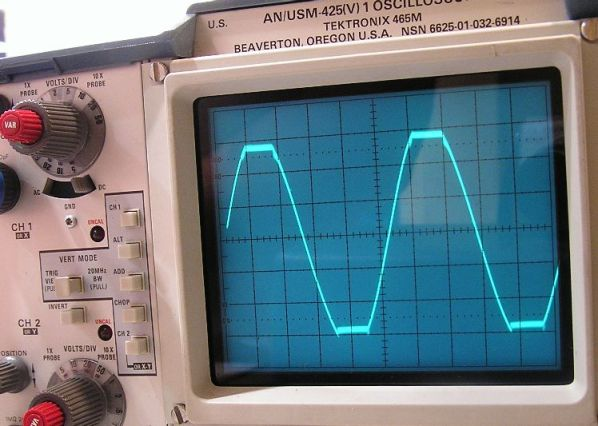
\includegraphics[width=0.7\textwidth]{clippingeffect.jpg}
  \caption{Photo showing the effect of clipping, a consequence of the overdrive or distortion effect.}
  \label{fig:clipping1}
\end{figure}


The consequences in the frequency domain are that the clipping effect creates more harmonics at high frequency than the signal without the clipping effect. \\

The clipping effect in signal processing happens when the amplitude is limited by a number and if during the processing the amplitude surpasses this limit, clipping happens because the value is then maxed to the maximum number that can be handled digitally. The maximum amplitude that can be handled is determined by the number of bits the system uses. The maximum number for a 16bit signed integers system is $\frac{2^{16}}{2} = 32768$ which means that if a value has an amplitude higher than this number the clipping effect occurs. \\

In any clipping technique, there is a creation of new harmonics. In the case of soft clipping, the new harmonics are multiples of the harmonics of the original tone. Valve Overdrive is a soft clipping technique for instance. In the case of hard clipping, they are not multiples which results to what is called intermodulation. Hard clipping usually happens when the harmonics of the original signal are not related by a multiple. Transistor overdrive is an example of hard clipping.  Effects of hard and soft clipping on the waveforms are shown in \autoref{fig:clipping2}.

In the previous paragraphs, distortion and overdrive has been explained as if they are the same effects. In fact, there is a small difference between the two. Distortion changes the original tone more than overdrive which means that distortion will generate more extra harmonics than overdrive and their amplitude tend to be higher. Overdrive effect has "cleaner" consequences on the final tone than distortion. Overdrive is often assigned to soft clipping while distortion is assigned to hard clipping.

\begin{figure} [htbp]
	\centering
  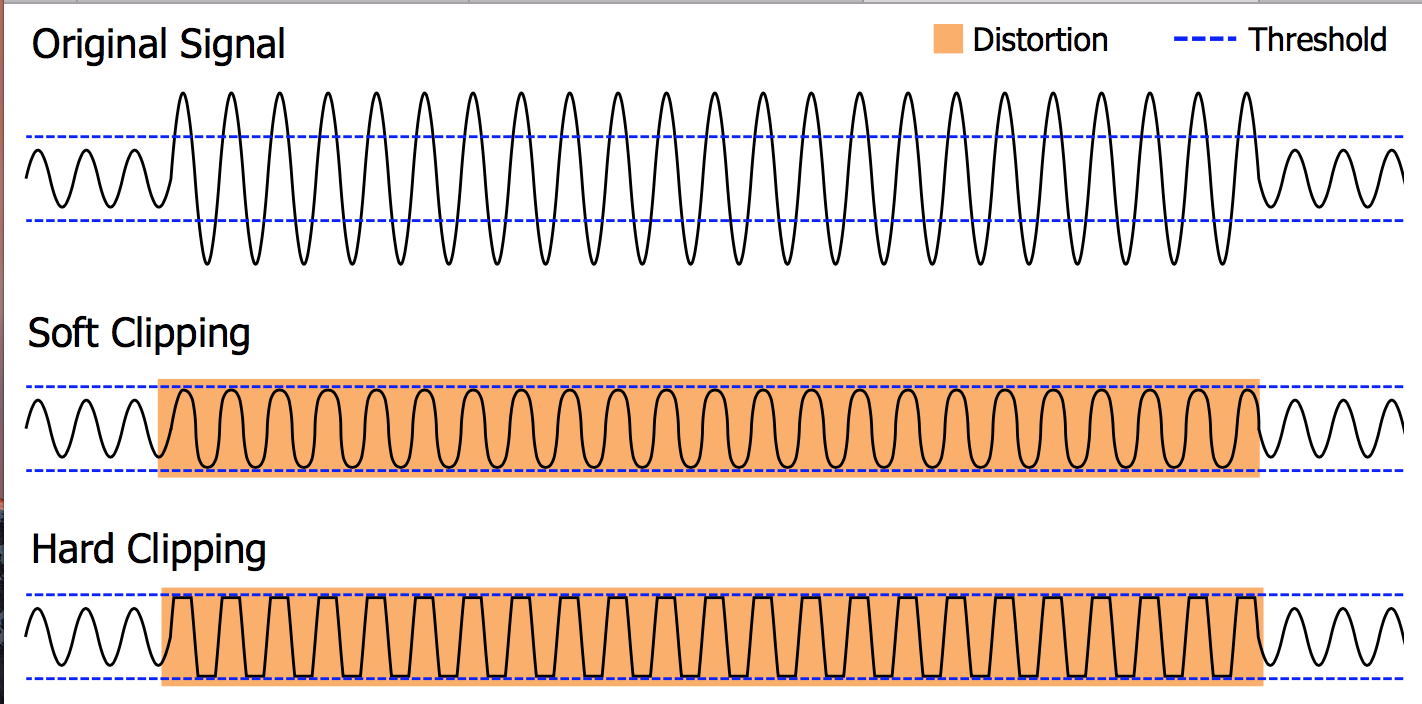
\includegraphics[width=0.7\textwidth]{softhardclipping.png}
  \caption{Photo showing the effect of hard and soft clipping, a consequence of the overdrive or distortion effect.}
  \label{fig:clipping2}
\end{figure}


